\documentclass[11pt, a4paper]{article}

\usepackage{graphicx}
\usepackage[a4paper,top=3cm,bottom=2cm,left=2cm,right=2cm,marginparwidth=1.75cm]{geometry}
\usepackage[english]{babel}
\usepackage[utf8x]{inputenc}
\usepackage{subfig}
\usepackage{float}
\usepackage{amsmath}
\usepackage{amssymb}
\usepackage{mhchem}
\usepackage{hyperref}
\usepackage{tikz}
\usepackage{cancel}
\usepackage{bm}

\graphicspath{ {./images} }
\newcommand*{\qed}{\hfill\ensuremath{\quad\square}}%
\newcommand*{\rad}{\ensuremath{\,\text{rad}}}
\newcommand*{\R}{\ensuremath{\mathbb{R}}}
\newcommand*{\C}{\ensuremath{\mathbb{C}}}
\renewcommand*{\Re}{\operatorname{Re}}
\renewcommand*{\Im}{\operatorname{Im}}
\renewcommand*{\epsilon}{\varepsilon}
\renewcommand*{\phi}{\varphi}
\renewcommand*{\d}{\text{d}}

\DeclareRobustCommand{\uvec}[1]{{%
  \ifcat\relax\noexpand#1%
    % it should be a Greek letter
    \bm{\hat{#1}}%
  \else
    \ifcsname uvec#1\endcsname
      \csname uvec#1\endcsname
    \else
      \bm{\hat{\mathbf{#1}}}%
     \fi
   \fi
}}

\makeatletter
\renewcommand*\env@matrix[1][*\c@MaxMatrixCols c]{%
  \hskip -\arraycolsep
  \let\@ifnextchar\new@ifnextchar
  \array{#1}}
\makeatother

\newtheorem{theorem}{Theorem}
\numberwithin{equation}{section}
\numberwithin{figure}{section}

%------------------------------------------------
%Templates for images and figures
% \begin{figure}[h]
%   \centering
%   \subfloat[caption 1]{{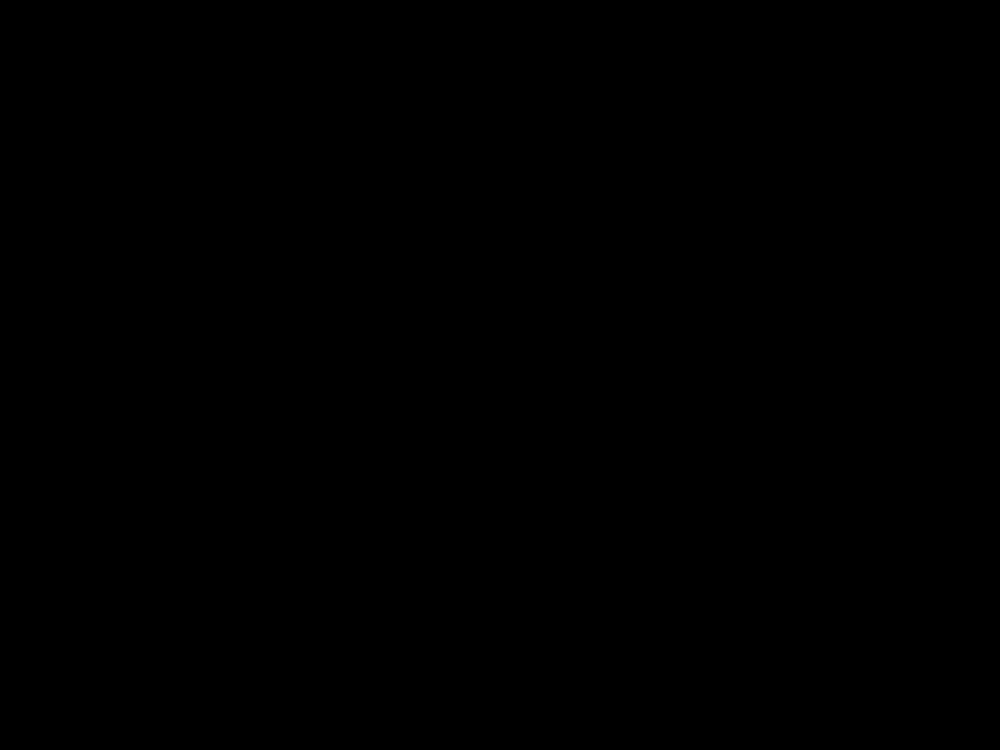
\includegraphics[width=30mm]{images/placeholder.png}}}%
%   \qquad
%   \subfloat[caption 2]{{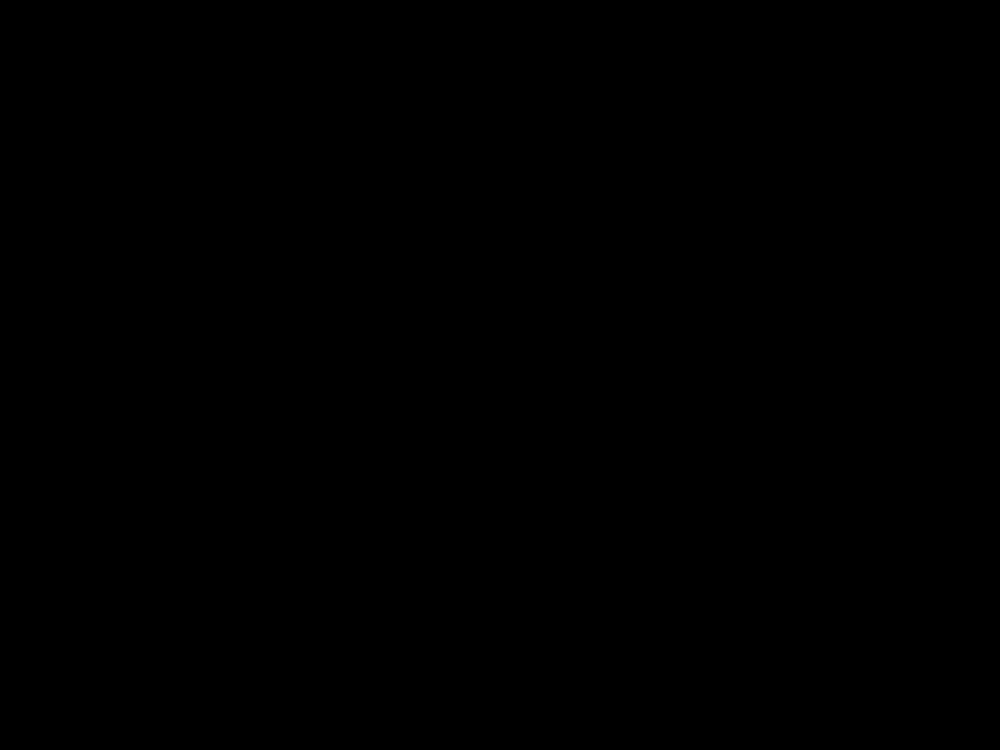
\includegraphics[width=30mm]{images/placeholder.png}}}%
%   \caption{Description}
% \end{figure}

% \begin{figure}[h]
%   \centerline{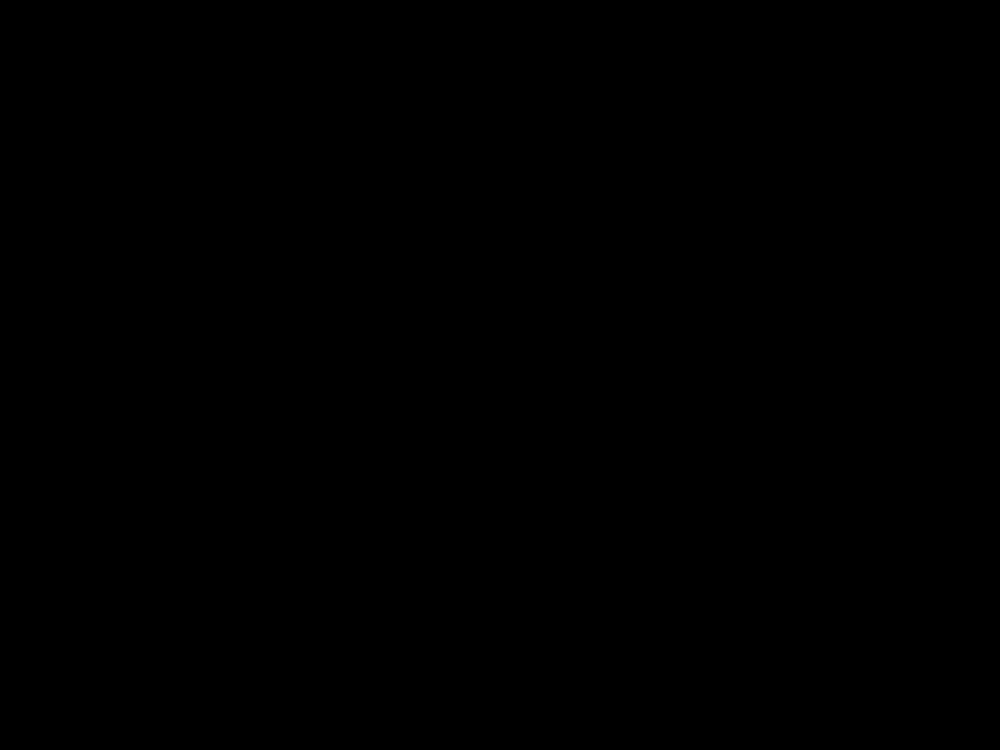
\includegraphics[width=50mm]{images/placeholder.png}}
%   \caption{Description}
% \end{figure}

%Template for a simple table 
%\begin{table}[h]
%   \caption{Description} %title of the table
%   \centering % centering table
%   \begin{tabular}{l rr} % creating three columns
%     \hline\hline %inserting double-line
%     & & \\ [0.5ex] % Insert half line vertical spacing
%     \hline % inserts single-line
%     & & \\ 
%     & & \\
%     & & \\
%     & & \\
%   \hline % inserts single-line
%   \end{tabular}
%   \label{tab:hresult}
% \end{table}
%-----------------------------------------------

\begin{document}
\setcounter{section}{4}
\section{Describing orientation in space}
\subsection{Rotation matrices}
A triad can be thought of as an orthonormal basis to a vector space. This means we can linearly transform a triad to another triad just by applying a matrix transformation. Since the triads are both orthonormal basis the determinant of this rotation matrix should also be equal to 1 as this would otherwise not preserve the fact that the basis vectors are all of length 1. Suppose $\vec{r}$ is just a random vector in $\R^3$ space. Furthermore suppose this space has 2 triads: triad $\mathcal{N}$ with unit vectors $\uvec{n}_1$, $\uvec{n}_2$ and $\uvec{n}_3$ in the $X$, $Y$ and $Z$ directions. The second triad is triad $\mathcal{B}$ which has the unit vectors $\uvec{b}_1$, $\uvec{b}_2$ and $\uvec{b}_3$ in the $x'$, $y'$ and $z'$ directions. Since we are dealing with 2 triads we can choose to represent our vector $\vec{r}$ in 2 ways:
\begin{equation}
  ^\mathcal{N}\vec{r} = 
  \begin{bmatrix}
    r_{n1}\\
    r_{n2}\\
    r_{n3}
  \end{bmatrix}
  \quad \text{or} \quad
  ^\mathcal{B}\vec{r} = 
  \begin{bmatrix}
    r_{b1}\\
    r_{b2}\\
    r_{b3}
  \end{bmatrix}
\end{equation}
Notice that the actual vector $\vec{r}$ stays the same no matter what triad we describe it in. We can translate a vector expressed in one triad to the same vector expressed in a different triad by taking the inner product of the vector and the unitvectors of triad $\mathcal{B}$ expressed in terms of triad $\mathcal{N}$. This looks a bit like:
\begin{equation}
  r_{b,i} = \,^\mathcal{N}\vec{r} \cdot \uvec{b}_i = |\vec{r}|\cos(\alpha_{ij})
\end{equation}
Instead of doing this to some random vector $\vec{r}$ we can also describe the unit vectors of different triads in terms of one another. In the case of expressing $\uvec{b}_1$  in terms of triad $\mathcal{N}$ we get:
\begin{equation}
  ^\mathcal{N}\uvec{b}_1 = 
  \begin{bmatrix}
    \uvec{b}_1 \cdot \uvec{n}_1\\
    \uvec{b}_1 \cdot \uvec{n}_2\\
    \uvec{b}_1 \cdot \uvec{n}_3
  \end{bmatrix}
  =
  \begin{bmatrix}
    \cos(\alpha_{x'X})\\
    \cos(\alpha_{x'Y})\\
    \cos(\alpha_{x'Z})
  \end{bmatrix}
\end{equation}
We can repeat this for are unit vectors in the triad and package them together in a matrix. When when we then apply this matrix to vectors in triad $\mathcal{N}$ it translates them into vectors expressed in triad $\mathcal{B}$ this means it's nothing but a change of basis matrix. From this we can also deduce that the inverse of the rotation matrix must be the matrix which translates triad $\mathcal{B}$ to triad $\mathcal{N}$, as this is nothing but changing the basis back into the original triad. The rotation matrix is given as:
\begin{equation}
  ^\mathcal{B}C_\mathcal{N} = 
  \begin{bmatrix}
      \cos(\alpha_{x'X}) & \cos(\alpha_{x'Y}) & \cos(\alpha_{x'Z})\\
      \cos(\alpha_{y'X}) & \cos(\alpha_{y'Y}) & \cos(\alpha_{y'Z})\\
      \cos(\alpha_{z'X}) & \cos(\alpha_{z'Y}) & \cos(\alpha_{z'Z})\\
  \end{bmatrix}
\end{equation}
Where the following relations holds:
\begin{equation}
  ^\mathcal{N}C_\mathcal{B} = \left(^\mathcal{B}C_\mathcal{N}\right)^{-1}
\end{equation}
A shortcut to this is that for symmetric matrices it's inverse and transpose are the same. Thus when we are dealing with a symmetric rotation matrix we find:
\begin{equation}
  ^\mathcal{N}C_\mathcal{B} = \left(^\mathcal{B}C_\mathcal{N}\right)^T
\end{equation}

\end{document}